\section{Work plan}

\subsection{Work breakdown structure} % for Draft B
\label{wbs}

The work breakdown structure is show in \tableref{work-breakdown}.

For each day allocated to a task (denoted ``1d,'') we allocated one hour of labour.
This is based on seven hours of work per week devoted to the project for each group member.

\begin{table}[!h]
	\centering
	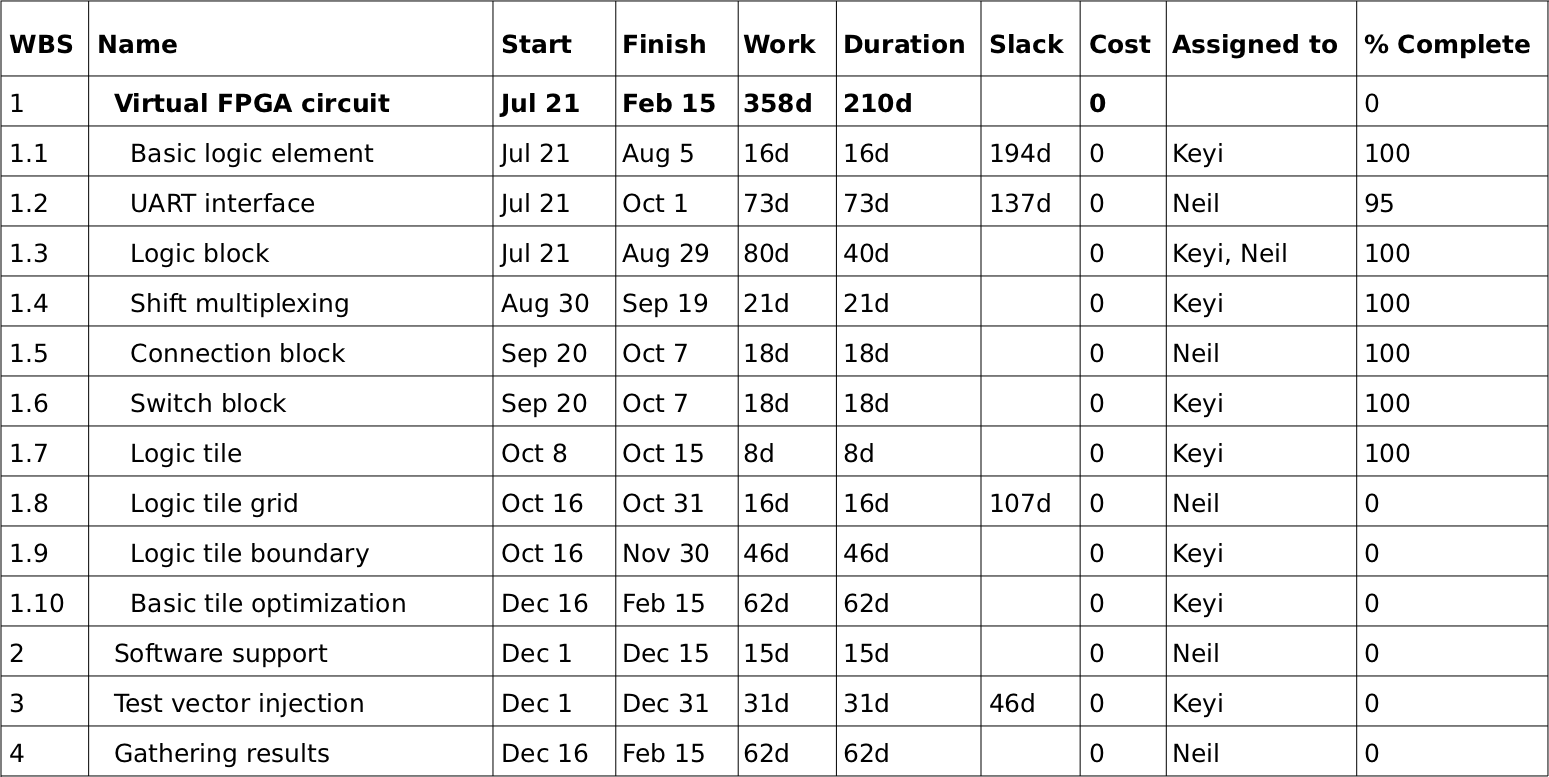
\includegraphics[scale=1.0]{wbs.png}
	\caption{Work breakdown structure}
	\label{work-breakdown}
\end{table}

Note that this work breakdown structure projects completion mid-February rather than mid-March to allow extra time for unforeseen engineering challenges.

\subsubsection*{Task Descriptions:}
\begin{enumeration}
	\item Overlay FGPA circuit: the hardware component of the project \
	\begin{itemlist}
		\item[1.1] Basic logic element: write Verilog sub-circuit of basic LUT element.
		\item[1.2] UART interface: write Verilog sub-circuit and a python program for bitstream programming via a serial cable.
		\item[1.3] Logic block: write Verilog sub-circuit of bundled logic cells with full input crossbars.
		\item[1.4] Shift multiplexing: write Verilog sub-circuits for efficient 2-layer and 3-layer multiplexers constructed from 32-bit shift registers.
		\item[1.5] Connection block: write Verilog for the connection block module.
		\item[1.6] Switch block: write Verilog for the switch block module.
		\item[1.7] Logic tile: write Verilog module of assembling the logic block, connection blocks, and switch block in a tile ready for tessellation.
		\item[1.8] Logic tile grid: assemble logic tiles into a grid to build the Overlay FGPA.
		\item[1.9] Logic tile boundary: handle input and output to and from the Overlay FGPA.
		\item[1.10] Basic tile optimization: tune the logic cell and routing for performance and area.
	\end{itemlist}
	\item Software support: write software to convert a VPR circuit to a bitstream for our circuit.
	\item Test vector injection: create a mechanism for test inputs to be transferred alongside and executed on the circuit, and for the results to be retrieved.
	\item Gathering results: Study and document the area overhead and performance of the circuits using different configurations.
\end{enumeration}


\subsection{Gantt chart} % for Draft B

\figref{gantt-chart} shows the proposed project plan corresponding to the work breakdown structure outlined in \sectref{wbs}.

\begin{figure}[!h]
	\centering
	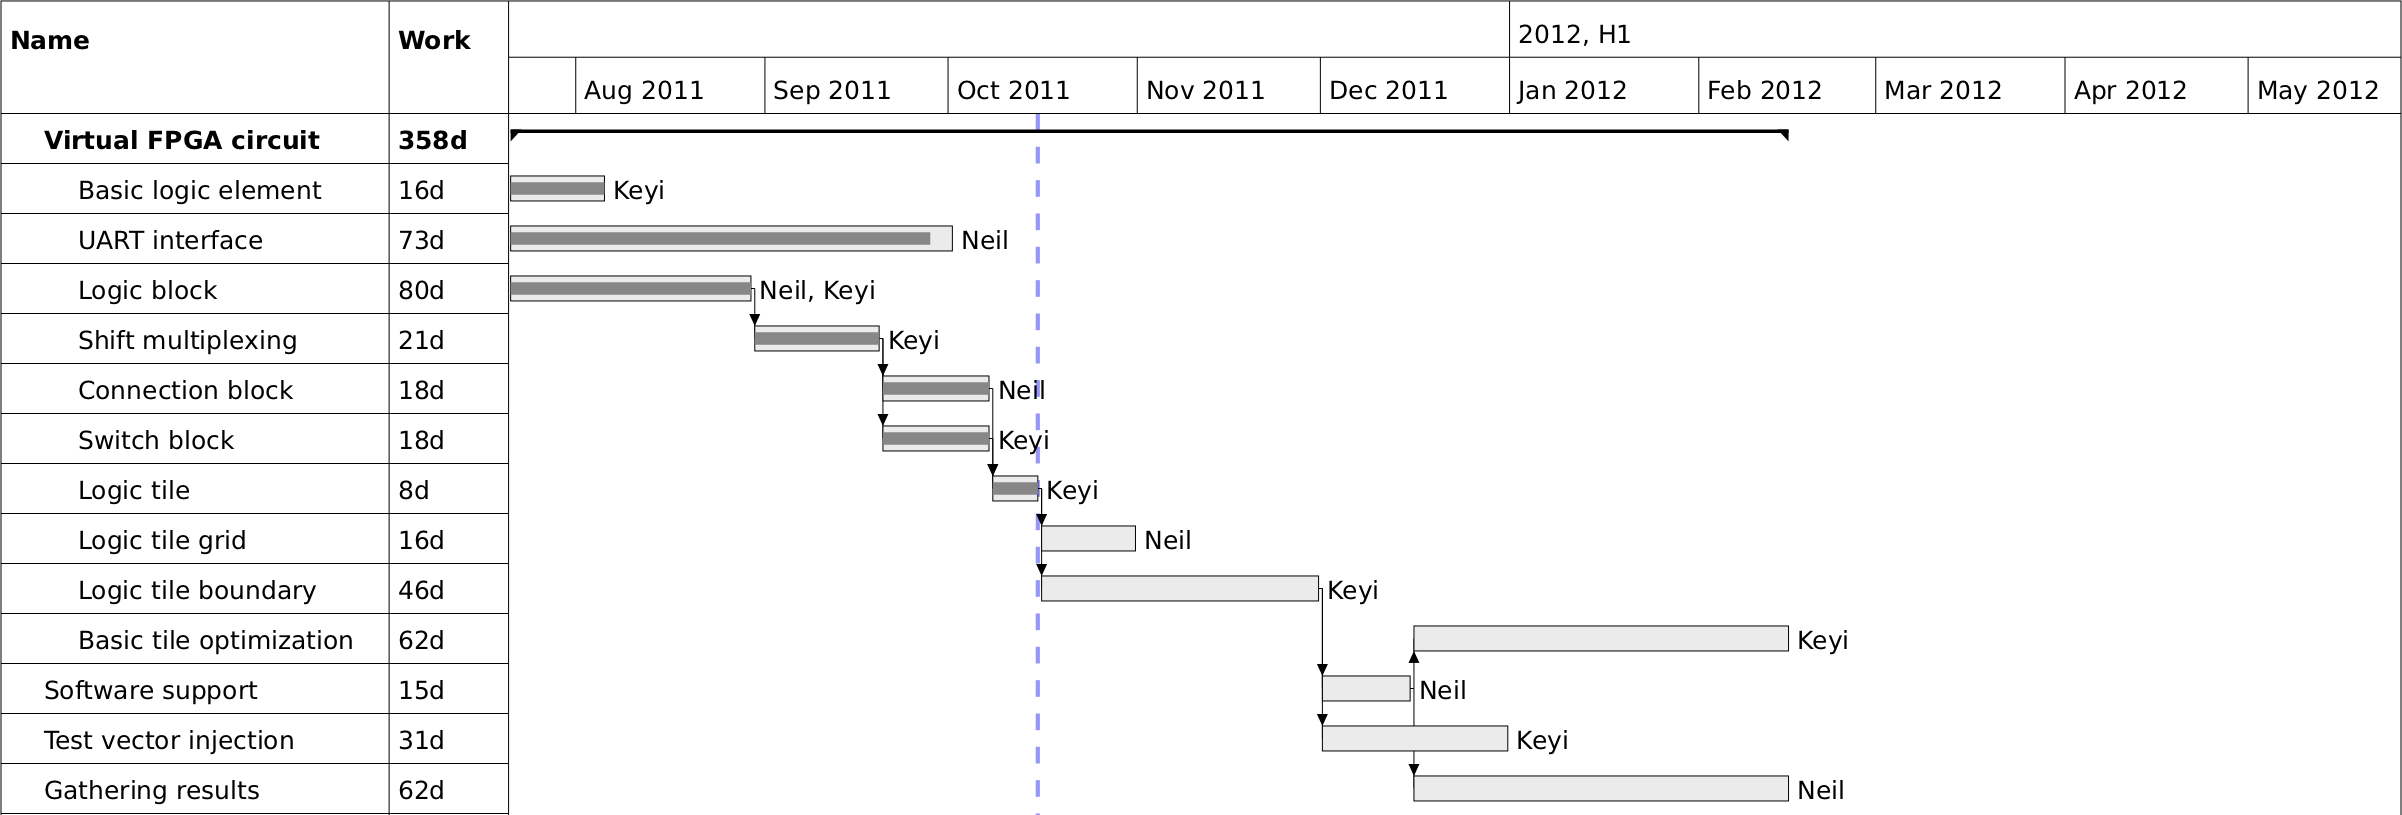
\includegraphics[scale=0.8]{gantt.png}
	\caption{Gantt chart showing project plan}
	\label{gantt-chart}
\end{figure}


\subsection{Financial plan} % for Draft B

% This section documents the costs of the project, which can include parts, computer
% hardware, software licenses, rental costs, etc. The Financial Plan consists of a budget
% table and an explanation of contingency arrangements if the necessary funding for the
% project is not acquired. You need not include your time, but should include "free" items
% that would cost money in industry, budgetted at $0.

The expenses of our project are documented in Table \ref{expenses-table}.
No additional financing is requested.

\begin{table}[!h]
	\centering
	\begin{tabular}{ | l | l | l | l | l | }
		\hline
		\textbf{Item} & \textbf{Source} & \textbf{Unit cost} & \textbf{Quantity} & \textbf{Total} \\
		\hline \hline
		FPGA development board & Supervisor & \$750.00 & 2 & \$0.00 \\
		ISE software licenses & Supervisor & & 2 & \$0.00 \\
		Personal computer & Students & & 2 & \$0.00 \\
		Serial cable & Students & \$5.00 & 2 & \$10.00 \\
		USB serial adapter & Students & \$2.00 & 2 & \$4.00 \\
		\hline
		Total & & & & \$14.00 \\
		\hline
	\end{tabular}
	\caption{Project expenses}
	\label{expenses-table}
\end{table}


\subsection{Feasibility Assessment}

% This section is meant to help your team, supervisor, and administrator assess the
% feasibility of your proposed project. This is not a marketing exercise: try to provide a fair
% and honest assessment of your proposal, balancing both its strengths and weaknesses.
% There is nothing wrong with identifying major deficiencies in your project; in some
% businesses, fewer than one in ten projects results in a commercially viable product.
% Identifying weaknesses and putting together a plan to address those weaknesses early on
% is a crucial part of the design process. It also helps your supervisor and administrator in
% their roles as effective mentors and guides.
% 

% Here are some of the key issues you should address in this section. Be brief - a sentence
% or two is probably enough to cover each issue. Also, these issues do not need to be
% addressed in any particular order and may be combined or reorganized to flow logically:
% Skills and resources:
% - What are the key skills, knowledge and resources you need for this project?
% - What portions have you already acquired and what portions are currently lacking?
%   How do you plan to obtain what you still need? Examples:
%    o From the web: free or open source software, technical standards, expert
%      forums
%    o From your supervisor: graduate researchers, lab space and equipment, etc.
%    o From the Design Centre (SFB520): facilities for making and soldering
%      printed circuit boards, used hardware from past design projects,
%      computers, test equipment, etc.

\subsubsection{Skills and Resources}

\begin{itemlist}
	\item Required Software \
		\begin{itemlist}
			\item ABC synthesis system to produce input for VPR - available online\footnote{ABC can be downloaded from: \url{http://www.eecs.berkeley.edu/~alanmi/abc/}}
			\item VPR placement and routing to produce our input data - available online\footnote{VPR 5.0.2 can be downloaded from: \url{http://www.eecg.utoronto.ca/vpr/}}
			\item FPGA vendor tools to implement our circuit: Xilinx ISE - licenses through supervisor
		\end{itemlist}
	\item Required Hardware \
		\begin{itemlist}
			\item FPGA development board - currently using Xilinx Virtex 5 from supervisor; Spartan 6 boards are also available from supervisor.
			\item Host computer to program the physical and overlay FPGAs - personal laptops
			\item Serial cable and USB adapter to interface with overlay FPGA - available at electronics stores
		\end{itemlist}
	\item Required Skills and Knowledge \
		\begin{itemlist}
			\item Verilog circuit design skills - gained from previous coursework and projects
			\item Knowledge of FPGA architecture - consulting with supervisor, studying recommended papers, software tools, and online resources
			\item VPR interfacing - consulting with graduate students who are working on VPR
		\end{itemlist}
\end{itemlist}


%
% Risk Assessment:
% In this section, describe the risks that the project could face (risk identification) and how
% you plan to deal with them (risk mitigation). An example of a risk would be that a
% particular component you envision might prove impossible to implement, and a
% corresponding risk mitigation strategy would be attempting to prototype the riskiest
% portion of your project as a feasibility assessment of the whole project. This would be
% coupled with a „fall-back‟ plan as to what you would do should this prototype fail.
% Merely, stating that risks will not occur, or that risks will be mitigated by working harder
% does NOT constitute back-up plan!
% This section should not be very long and you should focus on one or two real risks to
% your project (most likely technical risks but there could be others as well). Minor risks
% that will cause little disruption in schedule do not need to be addressed. Note that
% something that is technically challenging (or difficult to implement) may not necessarily
% be a significant risk to the project, if its failure does not affect the overall project goals or
% requirements (for example, the task may relate to a project objective for an additional
% feature, rather than a core requirement).
% Note: when addressing risks, focus on the most likely ones that are specific to your
% project. Some students ponder the risks of having a team member drop out of school, or
% losing all their work due to a computer crash. Such discussions aren't particularly helpful
% in planning your project. A more specific and effective series of questions might be
% - What happens to other components and to the project if component X that I‟ve
%     designed for my system fails to meet specifications or takes significantly longer to
%    develop?
% - Can I change the specifications, demonstrate a lower performance system, or
%   remove some features of my final design and still maintain the essential aspects of
%  my project?
% - What if our initial plan to build a real prototype proves unfeasible? Could we
%   demonstrate our design or part of our design using a computer model instead?
%  What would the limitations of this computer model-based prototype be? How
% would the project goal, requirements, and scope be modified to ensure that the
% new, redefined, project remains challenging?
% The key idea is to think of ways that you can modify the scope of your project so that you
% can show some partial success in realizing your Project Proposal by the end of the school
% year. More information and additional examples in [Design Notes, Chapter 11].
%
% Risk in Research Projects: Often, a research project will have above-average risk and
% this section may need to be longer. If the „Technical Design‟ section describes your
% intended initial strategy, this section should describe alternate directions that will be
% taken if experimental results indicate that the initial strategy is no longer what should be
% done. Here, the „risk‟ is that the experimental result or some intermediate result not be as
% expected (and the probability of this could be high) and the mitigation is the
% determination of an the alternate goal or an alternate route to the original goal.



\subsubsection{Risk Assessment}

\paragraph{Overlay FPGA implementation overhead}
\label{risk-size}

\begin{itemlist}
	\item Implementing the overlay's logic cells and interconnect on a physical FPGA will consume more area than the area consumed by an equivalent amount of logic cells and interconnect on the physical FPGA.
	\item If the overhead is too high, then we may not be able to fit enough logic cells for our benchmark circuits.
	\item For example, if a benchmark circuit consumes 5\% of a normal FPGA and the overlay has a 20x overhead, then the benchmark circuit may not fit on the overlay FPGA.
	\item Risk Mitigation strategies: \
		\begin{itemlist}
			\item Use a larger, more costly FPGA.
			\item Look for more architectural features in the physical FPGA that can be exploited to reduce the overhead of the overlay FPGA circuit.
			\item Use a smaller benchmark circuit for the proof of concept.
		\end{itemlist}
\end{itemlist}

\paragraph{Unbalanced timing}

\begin{itemlist}
	\item Logic cells in the overlay FPGA would ideally be arranged in a perfect grid, but we expect that the placement algorithm in ISE will not produce this arrangement on the physical FPGA.
	\item This means that the timing delay of two different cells to their respective ``right'' neighbours may differ.
	\item If this imbalance is too big, then the performance of the benchmark circuits may not be satisfactory.
	\item Risk Mitigation: Constrain a ``tile'' containing only one logic block to a rectangular shape, then tessellate it to form a grid, producing a more balanced design.
\end{itemlist}

